\documentclass{sigchi}

% Load basic packages
\usepackage{balance}  % to better equalize the last page
\usepackage{graphics} % for EPS, load graphicx instead 
\usepackage{mathptmx}
\usepackage[pdftex]{hyperref}
\usepackage{color}
\usepackage{booktabs}
\usepackage{textcomp}
\usepackage{microtype} % Improved Tracking and Kerning
\usepackage{ccicons}  % Cite your images correctly!
\usepackage{multicol}
\usepackage{color} 
\newcommand{\hl}[1]{\colorbox{yellow}{#1}}
\usepackage{xspace}
\usepackage{algorithm} 
\usepackage[noend]{algpseudocode} 
\usepackage{subcaption}
\usepackage{booktabs}
\def\algname{SPRING\xspace}
\DeclareMathOperator*{\argmin}{argmin}
\DeclareMathOperator*{\argmax}{argmax}
\usepackage{wrapfig, subcaption}

\usepackage{adjustbox}
\usepackage{tikz}
\usetikzlibrary{shapes,arrows,positioning} 
\tikzset{
	%Define standard arrow tip
	>=stealth',
	% Define arrow style
	pil/.style={
		<-,
		shorten <=0pt,
		shorten >=0pt,}
}

\floatname{algorithm}{Procedure}
\renewcommand{\algorithmicrequire}{\textbf{Input:}}
\renewcommand{\algorithmicensure}{\textbf{Output:}}


\usepackage{tikz}
\usetikzlibrary{decorations.pathreplacing,calc}
\newcommand{\tikzmark}[1]{\tikz[overlay,remember picture] \node (#1) {};}
\newcommand*{\AddNote}[4]{%
    \begin{tikzpicture}[overlay, remember picture]
        \draw [decoration={brace,amplitude=0.2em},decorate, thick, darkgray]
            ($(#3)!(#1.north)!($(#3)-(0,1)$)$) --  
            ($(#3)!(#2.south)!($(#3)-(0,1)$)$)
                node [align=center, text width=2.5cm, pos=0.5, anchor=west] {#4};
    \end{tikzpicture}
}%


% Paper metadata (use plain text, for PDF inclusion and later
% re-using, if desired).  Use \emtpyauthor when submitting for review
% so you remain anonymous.
\def\plaintitle{A Data-Driven Approach for Inferring Student Proficiency from Game Activity Logs  }
\def\plainauthor{Mohammad H. Falakmasir, Jos\'{e} P. Gonz\'{a}lez-Brenes, Geoffrey J. Gordon, Kristen E. DiCerbo}
\def\emptyauthor{}
\def\plainkeywords{Authors' choice; of terms; separated; by
  semicolons; include commas, within terms only; required.}
\def\plaingeneralterms{Documentation, Standardization}


% llt: Define a global style for URLs, rather that the default one
\makeatletter
\def\url@leostyle{%
  \@ifundefined{selectfont}{
    \def\UrlFont{\sf}
  }{
    \def\UrlFont{\small\bf\ttfamily}
  }}
\makeatother
\urlstyle{leo}

% To make various LaTeX processors do the right thing with page size.
\def\pprw{8.5in}
\def\pprh{11in}
\special{papersize=\pprw,\pprh}
\setlength{\paperwidth}{\pprw}
\setlength{\paperheight}{\pprh}
\setlength{\pdfpagewidth}{\pprw}
\setlength{\pdfpageheight}{\pprh}

% Make sure hyperref comes last of your loaded packages, to give it a
% fighting chance of not being over-written, since its job is to
% redefine many LaTeX commands.
\definecolor{linkColor}{RGB}{6,125,233}
\hypersetup{%
  pdftitle={\plaintitle},
% Use \plainauthor for final version.
%  pdfauthor={\plainauthor},
  pdfauthor={\emptyauthor},
  pdfkeywords={\plainkeywords},
  bookmarksnumbered,
  pdfstartview={FitH},
  colorlinks,
  citecolor=black,
  filecolor=black,
  linkcolor=black,
  urlcolor=linkColor,
  breaklinks=true,
}

% create a shortcut to typeset  headings
% \newcommand\tabhead[1]{\small\textbf{#1}}

% End of preamble. Here it comes the document.
\begin{document}

\title{\plaintitle}

\numberofauthors{4}
\author
{%
  \alignauthor{\mbox{\hspace{-1.85em}Mohammad H. Falakmasir$^{\star, \#} $\;\;\; Jos\'{e} P. Gonz\'{a}lez-Brenes$^\star$ \;\;\; Geoffrey J. Gordon$^\S$ \;\;\; Kristen E. DiCerbo$^\star$}\\
    \affaddr{$^\star$School Research}\\
    \affaddr{Pearson}\\
    \email{\{jose.gonzalez-brenes, kristen.dicerbo\}@pearson.com }\\
    }
  \alignauthor{\vphantom{Mohamamad Jose}
    \affaddr{$^\#$Intelligent Systems Program} \\
    \affaddr{University of Pittsburgh}\\
    \email{falakmasir@pitt.edu}\\
  }
  \alignauthor{\vphantom{Mohamamad Jose}
  	\affaddr{$^\S$Machine Learning}\\
	\affaddr{Carnegie Mellon University} 
  	\email{ggordon@cs.cmu.edu}\\
  }
}

  
\maketitle

\begin{abstract}
Traditional assessments are important in education because they allow collecting evidence about student progress. 
Unfortunately, they can be very tedious to the stakeholders.
In contrast, computer-based learning platforms provide the opportunity for invisible assessment by unobtrusively gathering students' digital learning footprints in order to track their progress and make inference about their relevant competencies.
We present a novel data analysis pipeline, {Student Proficiency Inferrer from Game data} (\algname), that allows modeling  game playing behavior in educational games.
Unlike prior work, \algname is a fully data-driven method that does not require costly domain knowledge engineering.
Moreover, it produces a simple interpretable model that not only fits the data, but also predics learning outcomes.
We validate our framework using data collected from students playing 11 educational mini-games.
Our results suggest that \algname is accurate to predict math assessments on a withheld test data (Correlation=0.55 , Spearman $\rho$=0.51).
\end{abstract}

\category{K.3.1}{Computer Uses in Education.}
{}
\keywords{Educational Games, Student Modeling, Stealth Assessment}

\section{Introduction}
Educational assessments are important because they collect evidence about  whether  the instructional goals are achieved or not.
Unfortunately, the process of  administering assessments is usually disconnected from the instructional environment, and  it is often  disruptive to the learning experience. 
In many developed countries, students now find themselves spending increasing amounts of time preparing and taking tests instead of learning~\cite{hofman2015rebalancing}.
For example, a  survey of the current state of testing in America revealed that students are taking an average of 113 standardized tests between pre-K and highschool~\cite{lazarin2014testing}. 
For these reasons, it is not surprising that the recent political climate and the general population have been weighing in on the question of whether students are being tested too much~\cite{lazarin2014testing}.


According to Evidence Centered Design (ECD)~\cite{mislevy2012design}, the goal of assessment is to characterize the strength of evidence regarding claims one wants to make about individuals or groups.
Therefore, the assessment process involves identifying, organizing, or creating activities for students in a way that we may observe that evidence.
An alternative to traditional summative assessment in computer based learning environments is invisible (or stealth) assessment~\cite{shute2013stealth},
where the evidence is unobtrusively gathered from leaners  interactions to understand claims regarding what students know and what they can do \cite{shute2009melding}.
Stealth assessment is also intended to reduce or eliminate test anxiety, while not sacrificing validity and reliability \cite{shute2008you}.

A promising opportunity for invisible assessment is using log data collected from educational games.
Unfortunately, engineering a system that parses log data is costly and time-consuming.
For example, prior work~\cite{shute2013stealth, shute2009melding} has relied extensively on domain expertise to define a \textit{Competency Model} in form of a Bayesian Network to describe the set of knowledge and skills involved in the learning environment.
They also used feature engineering on the performance data to build an \textit{Evidence Model} that expresses how student interactions with the system constitute evidence about competency model variables.

Our motivation is that invisible assessment from game data may become more accurate and cheaper to implement if the domain knowledge engineering could be automated by a data-driven process.
Game data is often logged  in a format that we call a \textit{slot and filler} structure.
In Table~\ref{tbl:log_example}, we show a simplified example of a real educational game log that uses slot and filler structure.
The slots are discrete sets of events that are initiated by the leaner.
Each slot may accept zero to multiple fillers. 
Each filler represents a value of a property of the slot event.
For example, a \texttt{Move Object} event  that represents the learner moving an object in the screen, may have an $x$ and $y$ coordinates as fillers to represent the target position in two-dimensional space.

\begin{table}[tbh]
	\begin{tabular}{@{}llll@{}}
		\toprule
		\textbf{Id}             & \textbf{User Id} & \textbf{Event Name} & \textbf{Event Data}        \\ \midrule
		1                       & ABC              & Game Start          & \{ \}                        \\
		2                       & ABC              & Move Object         & \{X:363,Y:82\} \\
		3                       & ABC              & Move Object         & \{X:361,Y:54\} \\
		4                       & ABC              & Open Toolbox        & \{\}        \\
		4                       & ABC              & Activate Tool        & \{tool:gluumi\}        \\
		5                       & ABC              & Use Gluumi        & \{sizeGluedTo:8,sizeNew:9\} \\        
		\multicolumn{1}{c}{...} &                  &                     &                            \\ \bottomrule
	\end{tabular}
	\caption{An example fragment of a log from an educational game. \label{tbl:log_example}}
\end{table}


Conventional machine learning algorithms cannot input slot and filler data, as they  usually work with data structures called \textit{feature vectors} or \textit{sequences}.
Prior research ~\cite{sequences} have compared these data structures in educational applications.
A feature vector representation requires mapping an observation onto a fixed number of features.
It is not obvious how to best map sequences of student actions that can be of an arbitrary length into a feature vector that needs to be of a predetermined dimension.
Traditional feature vector classifiers (like logistic regression or decision trees)  that are used in off-the-shelf data mining packages, such as Weka \cite{hall2009weka}, cannot  use slot and filler data as input. 
In contrast, machine learning algorithms that allow sequential representations, like Hidden Markov Models (HMM), require a parametric model with the same number of dimensions for all of the observations.
This does not occur in slot and filler structures.
For example,  in Table~\ref{tbl:log_example}, the \texttt{Move Object} slot requires \texttt{x} and \texttt{y} fillers, while the \texttt{Use Gluumi} slot requires only \texttt{size} fillers.

In this paper, we propose \textit{Student PRofficiency INferrer from Game data} (SPRING), a novel data analysis pipeline that models game playing behavior.
\algname first receives the interaction data in slot and filler format as input and generates a sequence of abstract observations by employing an unsupervised clustering method. 
The next step of the pipeline employs non-parametric extensions of HMMs in each game level to build a statistical representation that is generalizable across multiple game levels. 
The HMM models captures patterns of student interactions as a set of unobserved states, each state related to the abstract observations through a probability distribution. 
Finally, the last stage of the pipeline builds a regression model using features extracted from the HMMs of each game level to predict the student post-test scores.
We demonstrate the effectiveness of our approach on real student game playing data.
Our experiments suggest that \algname can be used to predict student proficiency.
The method is purely data-driven and learns parameters from student data without assuming a model. 
The only assumption here is that high- and low-performing students interact differently with the game environment and \algname is able to capture these differences.
%Moreover, we use a fairly straight forward data-driven process to replace the labor intensive task of carefully designing a game-specific model (by experts).
The more student data is available, the better parameter estimation we can perform and the learned HMM as a graphical model can be used in post-hoc interpretations by domain experts to gain insight into students' interaction patterns.

\section{Background}
The potential of computer games for educational purposes has been of interest since nearly the beginning of videogames. Unlike video games, which focus on creating an entertaining experience for the user, educational games require principles and strategies that engage students while maximizing their learning gain. Therefore, studying student interactions is a crucial step toward understanding their learning process and improving the game environment in the future.

There have been numerous attempts among the educational research community to develop analytic methods and build predictive models based on the data from educational games. \textit {Rumble Blocks}  is a physics educational game designed to teach basic concepts of structural stability and balance to children in grades K-3 (ages 5-8 years old). Harpstead et al. \cite{harpstead2014using}, studied the alignment of game to its target learning goals by examining whether student solutions follows the targeted principals. They employ clustering techniques on the individual solutions created by actual students and use principle-relevant metric (PRM) to measure how closely the representative solution embodies a specific targeted principle. The results demonstrated a misalignment between the feedback provided to students and the targeted knowledge.

\textit {Battleship Numberline} is another educational game for understanding fraction using number line estimation. Students attempt to explode target ships and submarines by estimating numbers on a number line. Lomas et al. \cite{lomas2013optimizing} performed a large-scale online experiment in order to study the effect of challenge on player motivation and learning. They presented different configurations of the game for different groups of students and used a combination of time spent and challenges attempted as a measure of engagement and the average success rate of each design configuration as a measure of challenge. The results showed a linear correlation between challenge (difficulty) and engagement, meaning the easier the game, the longer students played.

\textit {Refraction} is another educational game for learning about fractions by splitting laser beams into fractional amounts to target spaceships by avoiding asteroids. Liu et al. \cite{liu2013predicting}, created an ensemble algorithm that combines elements of Markov models, player heuristic search, and collaborative filtering techniques with state-space clustering in order to predict player movements on last game-level based on the history of movements in previous game levels. Lee et al. \cite{lee2014learning} extended the former framework by building state-action graph and using feature selection techniques to reduce the number of features for each state. To ensure extensibility, they also tested the framework on another game \textit {DragonBox} and reported improvement over a Markov predictor.

\textit {Quantum Spectre} is a more complex puzzle-style educational game designed for high school students to learn optics. Eagle et al. \cite{eagle2015measuring} used interaction networks (IN) to visualized and derive insight into students' problem solving behavior and common misconceptions. They used data from 195 students in 15 classes and created the full IN of every state and possible actions for each game level. Next, they used clustering to reduce the state-action space into a high level visualization of how each student progress through the puzzle and classify each student interaction into four categories: correct, placement error, rotation error, and puzzle error. 
Finally, they picked a smaller set of students (n=10) and used a linear regression model to predict the post-test results.
The results shows a direct negative relationship between science-related game play errors and the post-test scores.

\section{SPRING Algorithm}

\algname is designed in a way that can capture sequential decision making process of students in a way that is representative of their mastery with minimum reliance on expert knowledge. 
Our data analysis pipeline receives raw data of student interactions with the different levels of educational game in slot and filler format along with their post-test results and creates a regression model for predicting the post-test scores. 
Algorithm~\ref{alg:spring} describes the three main steps of our pipeline: discretization,  sequence modeling, and regression.
The discretization step transform slot and filler observations into multinomial indicators that are used as evidence for learning.
The sequence modeling step, learns a representation from data in form of a Hidden Markov Model for high- and low-performing students.
The regression step, uses the likelihood of student sequences in each game level as a feature to predict the post-test results.
We now explain the different steps in detail.

\begin{algorithm}[ht]
\begin{algorithmic}[1]
\Require: A log file $\mathbf{L_{g,s,t}}$ of slot-and-filler structure for each game $g$ and student $s$ (indexed by time $t$), and results from a student assessment $y_s$, number of performance clusters $K$, number of latent states $H$.
\For {each  game $g$}  \tikzmark{disctop}
	\For {each slot $z$}
		\State $\mathbf{D_{g,s,t}} \leftarrow$  Discretize\_Fillers($\mathbf{L_{g,s,t}}, z$) 
	\EndFor 
	\State  $\langle s, c \rangle \leftarrow$  Cluster\_Students($y_s, K$)  \tikzmark{discbot}
	\For {each student performance group $c$} \tikzmark{seqmodtop} \tikzmark{right}
		\State  $\mathbf{D_c} \leftarrow \mathbf{D_{g,s,t}}$ where $s \in \langle s, c \rangle$  
		\State$\theta_{g, c} \leftarrow$  Learn\_HMM($\mathbf{D_c}, H$) 
	\EndFor\tikzmark{seqmodbot}
\EndFor 
\For{each sequence $d$ in $\mathbf{D_{g,s}}$}  \tikzmark{regtop}
	\State  $\phi_{g,s} \leftarrow$  Extract\_Features($d,\theta_{g,c}$)  
\EndFor
\State Learn a model that predicts $y_s$  from $\phi_{g,s}$ 
\tikzmark{regbot}
\end{algorithmic}
%\AddNote{disctop}{discbot}{right}{\small{Discretization}}
%\AddNote{seqmodtop}{seqmodbot}{right}{\small{Sequence Model}}
%\AddNote{regtop}{regbot}{right}{\small{Feature Vector Model}}
\caption{The SPRING algorithm\label{alg:spring}}
\end{algorithm}



\subsection{Discretization}
We now describe how we discretize
the slot and fillers,  (\S~\ref{sec:filler_disc}) 
and the student performance (\S~\ref{sec:student_disc}).

\subsubsection{Slot-Filler Discretization}
\label{sec:filler_disc}

\begin{algorithm}[ht]
	\begin{algorithmic}[1]
		\Require: $L_{g,s,t}$, Sequence of slot-and-filler observations in game level $g$ and student $s$, slot $t$
		\Procedure{Discretize\_Fillers}{$\mathbf{L_{g,s,t}}, z, g$}
		%\State \Comment Get filler data for a game $g$ and slot $z$
		\State{$\mathbf{F_{s,t} } \leftarrow$  get\_fillers($\mathbf{L_{g',s,t}}$), where $g' = g$}
		
		\State{ $\langle \mathbf{F_{s,t}}$ , clustersIDs   $\rangle \leftarrow$ Cluster($\mathbf{F_{s,t}}$) } 
		\State{model  $\leftarrow$ learn\_classifier(filler\_values, clustersIDs) }
	
		\State
		\For{each student $s'$}	
				\For{each time step $t'$}
					\If {$z$ == slot($L_{g,s',t'}$)}
						\State { $\hat f \leftarrow$  model.predict(filler($ L_{g,s',t'} $)) }
						\State {$d  \leftarrow $ \text{concat}(z, $\hat f$) }
						\State{$\mathbf{D_{g,s',t'}} \leftarrow  d$} 
					\EndIf
				\EndFor
		\EndFor
		\State \Return{ $\mathbf{D}_{g,s,t}$ }
		\EndProcedure
		
	\end{algorithmic}
	\caption{The Discretization Step of \algname \label{alg:discretize}}
\end{algorithm}


Algorithm~\ref{alg:discretize} describes the method we use to discretize fillers.
The input is time-ordered student interactions in slot-and-filler format for a single slot $z$ and game $g$.
The purpose is to transform the slot and filler observations into a discrete (multinomial) observations appropriate for sequence modeling.
For example, consider the \texttt{Move Object} slot from Table~\ref{tbl:log_example}.
We wish to transform the different possible fillers into discrete units.
Figure~\ref{fig:screenshot} shows a screenshot of a minigame that generates  \texttt{Move Object} slots.
The purpose of this game is for learners to move ice cubes from the mountain top onto the two designated areas to prevent the Yeti from crossing the wall.
In Figure~\ref{fig:clustering} shows a scatterplot of the $x$ and $y$ fillers aggregating across 77 students.

\begin{figure}[ht]
 \centering
\begin{subfigure}[t]{.5\textwidth}
	\centering
	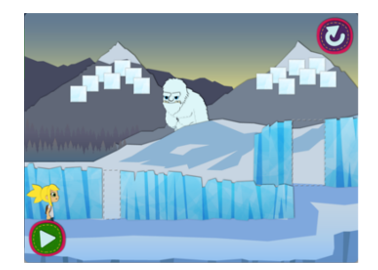
\includegraphics[width=0.9\columnwidth]{figures/glacier_screenshot.png}
	\caption{Screenshot of game level 2, \textit {None Shall Pass!} \label{fig:screenshot}}
\end{subfigure}
\begin{subfigure}[t]{.5\textwidth}
	\centering
	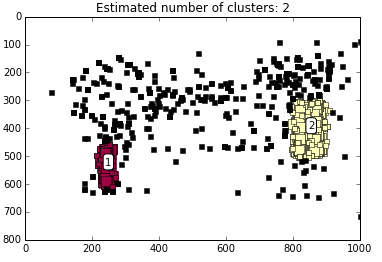
\includegraphics[width=0.9\columnwidth]{figures/glacier_positions.png}
	\caption{Clusters found using DBSCAN method. We transform each movement action into corresponding cluster id during the discretization step. \label{fig:clustering}}
\end{subfigure}
\caption{Analysis of the  \texttt{Move Object} slots and fillers from the \textit{None Shall Pass!} mini game\label{fig:figurecluster}}
\end{figure}

In order to transform the slot and filler observations into discrete events, we use an unsupervised clustering algorithm for the fillers of each slot.
For example, in Figure~\ref{fig:clustering}, we have three clusters,  cluster one and two (red and yellow respectively) that represent frequent movements, and cluster zero (black) that represents ``outlier'' movements.
We speculate that the outlier group is a result of either technical glitches in the gaming environment or student misconceptions.
To build discrete events we use the  concatenation of slot and cluster labels as a  observations in the sequence modeling phase.
For example, instead of modeling from an infinite  domain like ``\texttt{Move Object $\langle x:363, y:83 \rangle$}",
we use a number of discrete observations like ``\texttt{Move Object Cluster 1}".

The specific clustering algorithm we used  for learning a \algname model is DBSCAN~\cite{ester1996density}.
In our preliminary experiments we tried other unsupervised methods, but  we found DBSCAN easier to use because it can find arbitrarily shaped clusters and does not require one to specify the number of clusters in advance.
The time complexity of DBSCAN is $O(n \log n)$ (n = the number of data points) and there are recent parallelized implementations that are scalable \cite{patwary2012new,dai2012efficient}.

Clustering algorithms, like DBSCAN, often can only discretize observations in the training dataset, and would not generalize to unseen fillers.
To work around this limitation, we trained a classifier for transforming any filler into a cluster label. 
In particualr, we used a K-Nearest neighbor (K-NN, n=5) classifier because similar to DBSCAN, it uses an euclidean distance function as a similarity metric.
The classifier is trained to identify a cluster label using the fillers as predictors.
The K-NN classifier might not be the best choice for fillers in the outlier cluster. 
However, our preliminary experiments using cross-validation showed that it has enough discriminative power to distinguish the outlier fillers from other clusters.


\subsubsection{Student Performance Clustering}
\label{sec:student_disc}

In order to find an interpretable model that describes the behavior of different groups of students, researchers often use unsupervised and non-parametric methods.
However, since we are particularly trying to find patterns among students that is predictive of their post-test performance, we used the median of post-test scores to divide students into two groups. 
In each game level, we place the students who received a post-test score below or equal to the median in the low-performing group and the students who received a post-test score higher than the median in the high-performing group.
Due to the small number of students in our dataset, particularly in the later game levels, we only used two clusters. 
We hypothesized that students in difference performance groups play the game differently. 
Our sequence modeling phase should be able to capture these differences by learning the interaction patterns of each group in different game levels.

\subsection{Sequence Modeling}
Once we have transformed the slot-and-filler structure into sequences of discrete observations, we can start looking for sequential patterns among different performance groups in each game level.
Hidden Markov Models are a popular statistical tool for analyzing sequential pattern. 
Given the sequence of student actions (observations), we aim to infer a set of unobserved (latent) states, which describe the process that generated the observations, along with statistical patterns that can describe and distinguish those states.
However, learning the ``best" value for number of states ($H$) is a difficult problem in practice. 
There has been considerable prior work on this problem that used penalized likelihoods \cite{rabiner1989hmm}, Monte-Carlo cross-validation \cite{smyth1996clustering}, and mixture of HMMs \cite{smyth1997clustering}.
We used the Hierarchical Diriclet Process HMM (HDP-HMM) \cite{fox2008hdp}, which allows state spaces of unknown size to be learned from data. 
HDP-HMM defines a \textit{hierarchical Dirichlet process} prior on transition matrices over countably infinite state spaces and is able to make a principled choice of how many states it needs based on the complexity of its training data. 
For details on training methods please refer to \cite{fox2008hdp}.

We used the output of the discretization step (2D array of multinomial observations) and trained two HDP-HMMs, one for high-performing and the other for low-performing students in each game level. The two models can be considered as a stochastic representation of the sequence of actions and we can use them to infer the likelihood of any arbitrary sequence as a feature for the regression step. 

\subsection{Feature Vector Modeling}

For each student $s$ in each game level $g$, we calculate the difference between ($d_{s,g}$) the likelihood of belonging to the high- and low-performing group.
We calculate this likelihood by estimating the Forward-Backward probabilities  on each student sequence of actions  based on the two HMMs parameter we estimated (whether the student is in the high performing group or in the low performing group) and using a hyperbolic tangent function in order to convert it to a value between -1 and 1: 
\begin{equation}
d_{s,g} = tanh[ K * (\theta_{g, \text{high}} - \theta_{g, \text{low}})]
\end{equation}

We use  a linear regression model for predicting the post-test scores:

\begin{equation}
\hat {y_s}(\beta) =   \sum_g \beta_g \cdot d_{s,g}  + \beta_0
\end{equation}

Here, $\beta_0$ is just an intercept for the  model.  
We optimized the parameters of the model using a 5-fold cross validation on our development set.
We experimented with different regularization methods, but only report LASSO \cite{tibshirani1996regression} as it worked best in our preliminary comparisons:
\begin{equation}
\beta^* = \argmin_\beta || y_s - \hat{y_s}(\beta)  ||_2 + \lambda \cdot || \beta ||_1
\end{equation}


\section{Empirical Evaluation}

\subsection{Game Environment}
\textit {Alice in AreaLand} is an educational game developed as a part of Pearson Insight Learning System \footnote{http://researchnetwork.pearson.com/learning-science/insight-learning-system}. 
It focuses on teaching and assessing geometric measurement, specifically the understanding of area, among 6\textsuperscript{th} grade students. 
The game targets three main stages in the development of area: 1) area unit iteration, 2) use of unit squares to measure area, and 3) use of composites to measure area. 
The current version has 12 game levels. 
A simple student scenario involves covering a 2D area with smaller unit squares placed end-to-end in non-overlapping fashion, combining the single squares into rows or columns, and then determining the number of rows or columns needed. 
Figure~\ref{fig:figurekracken} shows a screenshot of one game level.

\begin{figure}
	\centering
	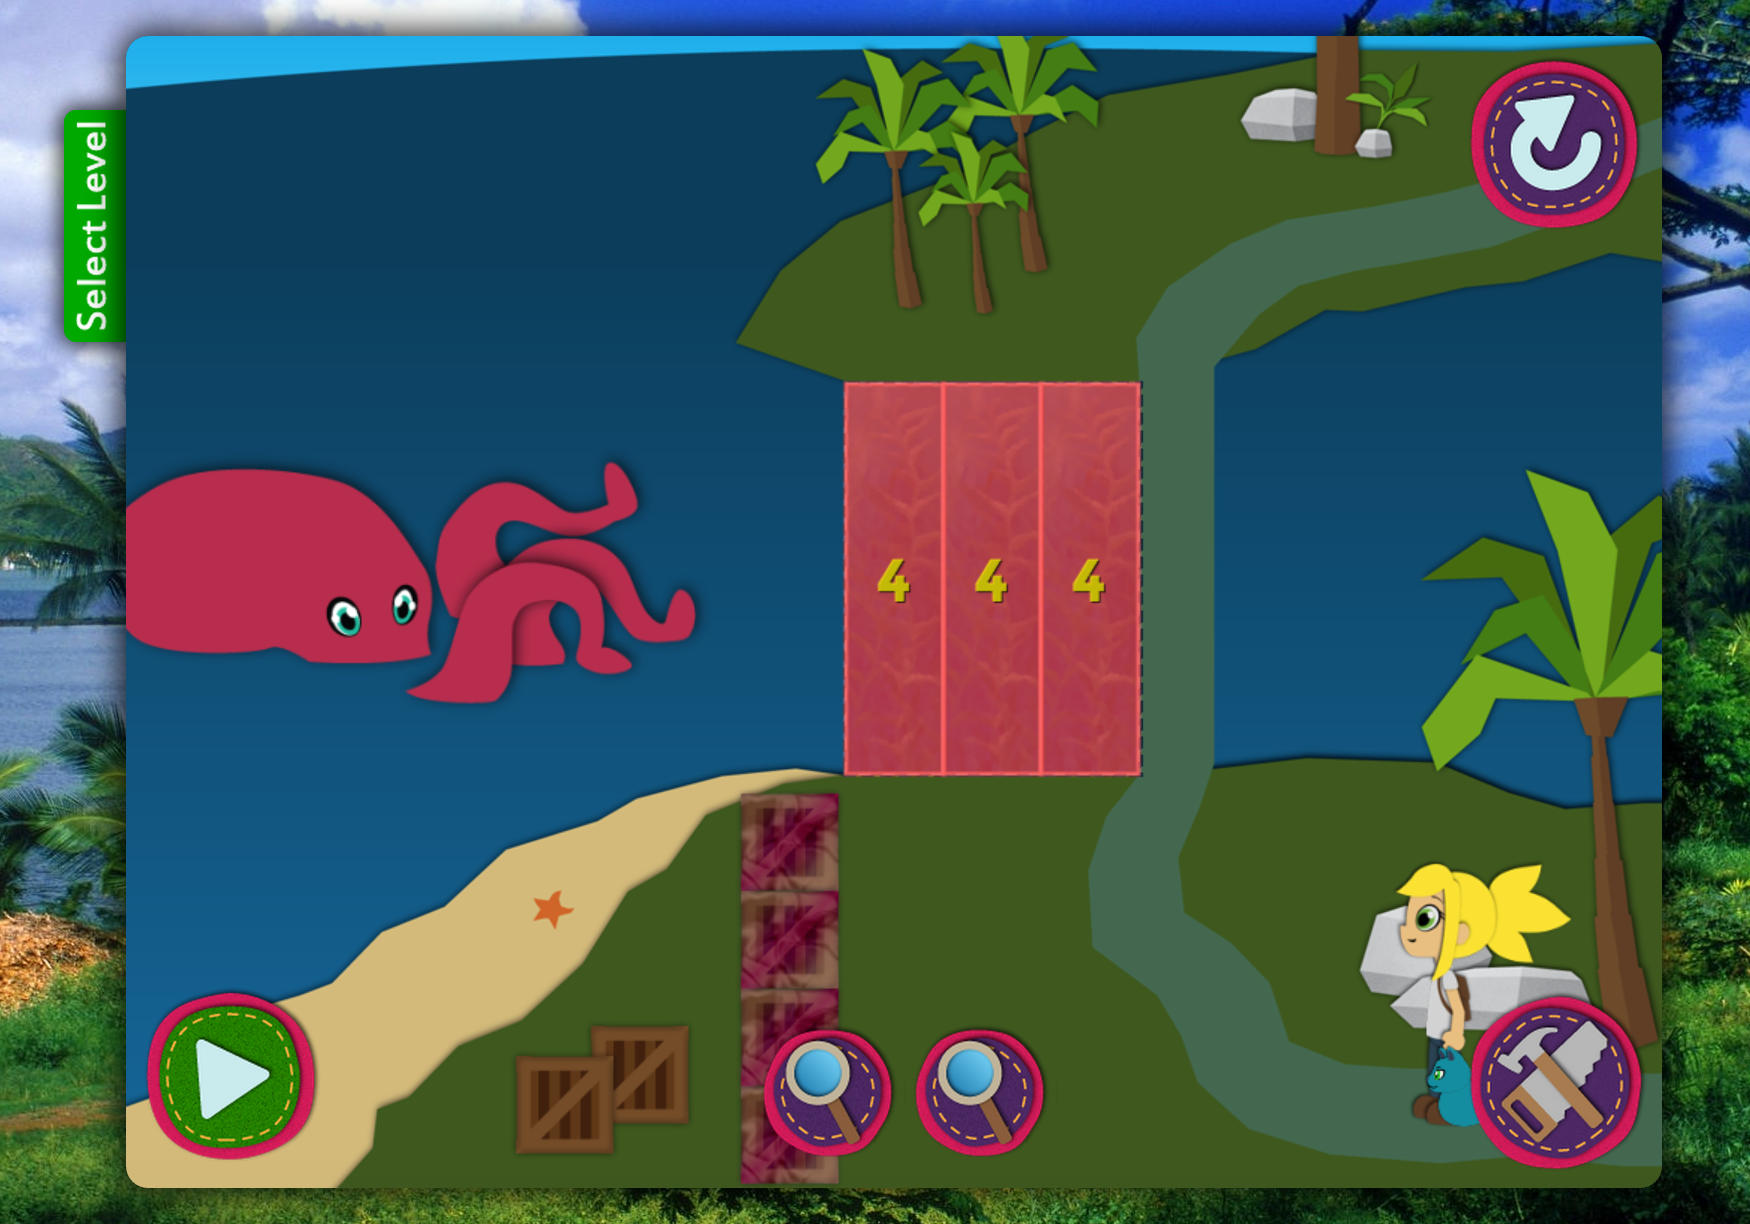
\includegraphics[width=0.9\columnwidth]{figures/kracken}
	\caption{A screenshot of hint provided in game level 11, \textit {You Kraken Me Up!}, in \textit {Alice in AreaLand}. Students should combine four squares into a column and create three copies of the column to cover the designated area and prevent the octopus from attacking \textit {Alice} while she crosses the bridge.}~\label{fig:figurekracken}
\end{figure}

Throughout the game,  \textit {Alice} is accompanied by \textit {Flat Cat} -- an assistant character who provides feedback and scaffolding to the player in the beginning of each game level and upon request when students push a hint button (represented by two magnifiers at the bottom center of Figure ~\ref{fig:figurekracken}). 
Earlier game levels are designed for students to learn about area unit iteration and usually require them to cover a number of predefined areas with unit squares (not necessarily in a non-overlapping fashion). 
By advancing through game levels, students are presented with three tools: \textit {Gluumi} for combining unit squares by gluing them together; \textit {Multy}, for making copies of different objects; and \textit {Esploda} for breaking compound shapes into single units.  
There is no limit for completing a game level regarding time or number of actions students may execute. 
The students press the \textit {Go Alice} button (bottom left corner of Figure~\ref{fig:figurekracken}) if they deem their performance to be satisfactory for \textit {Alice} to proceed. 
Based on the covered area and the arrangement of the tiles, they either advance to the next level or receive a feedback and stay in the same level.

\subsection{Dataset} 
Our dataset consists of time-stamped interactions of 129 students in 11 game levels.
We did not use the data from one of the game levels due to technical issues.
For 77 students, we also have post-test scores from a paper-based exam with 20 questions in the 3 skills of geometric measurement.
The post-test score ranges from 0 to 18 (out of 20) with the mean equal to 7.81 and standard deviation of 4.36. 
In total, there are 88,458 events recorded in the dataset from 1,510 game sessions, meaning that student tried some of the game levels for multiple times.
Based on the ECD framework, beginning levels only involve area unit iteration skill and the other skills and related features are gradually added to the later game levels.
Figure \ref{fig:frequency} shows the frequency of different events in each game level. As depicted in Figure \ref{fig:frequency}, the student interactions with the system in all game levels is dominated by movements.

\begin{figure}
	\centering
	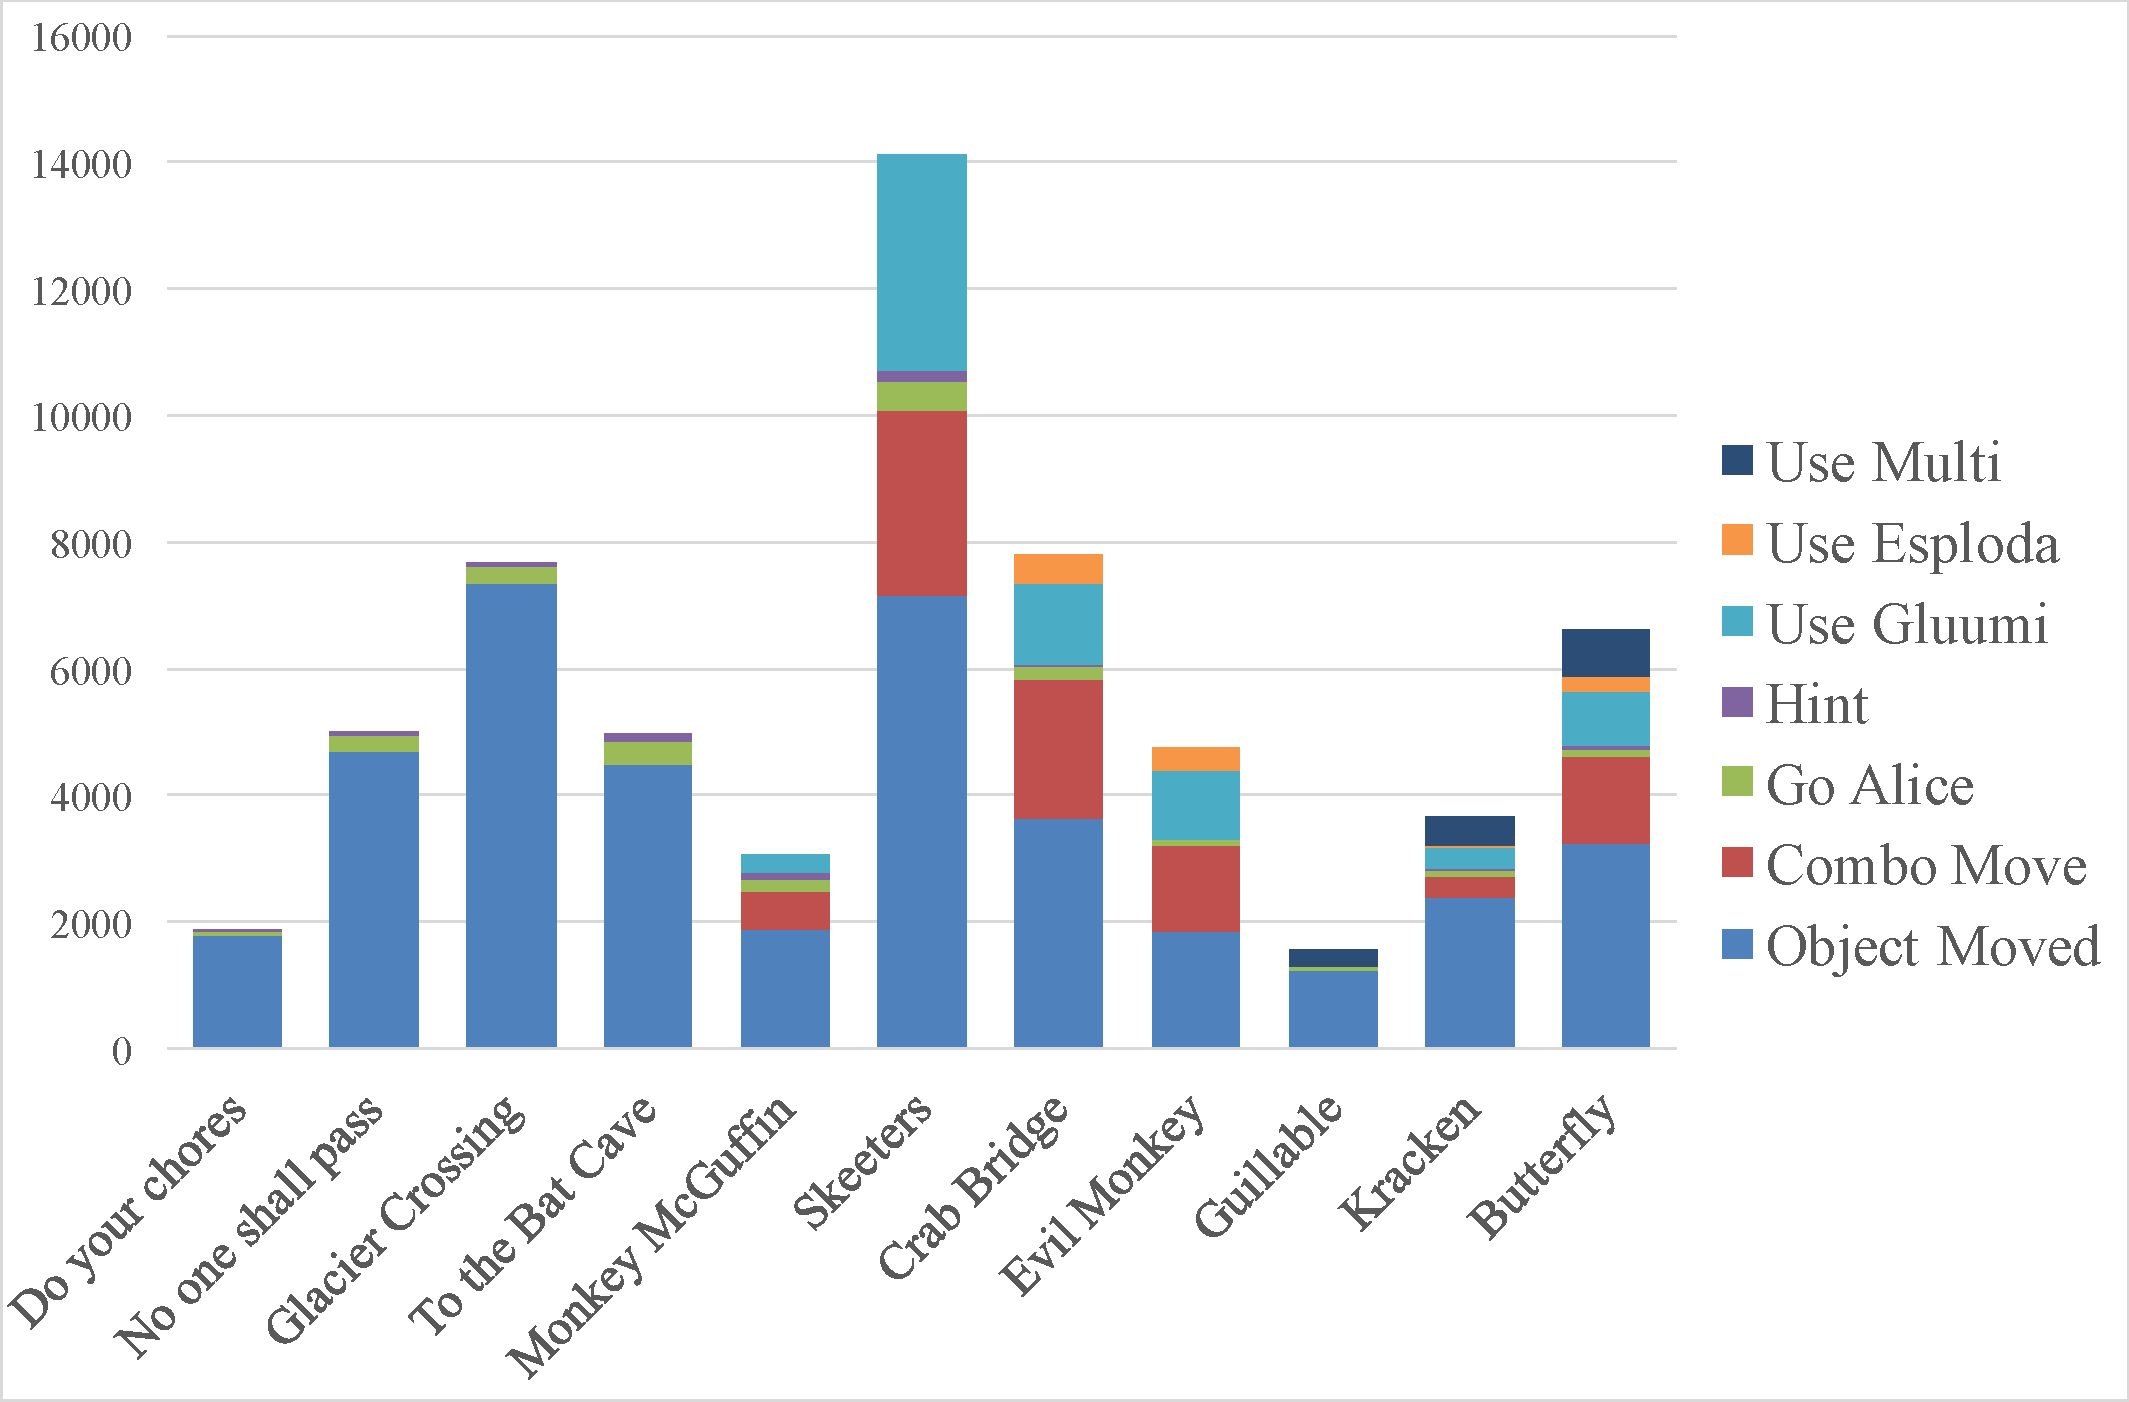
\includegraphics[width=0.9\columnwidth]{figures/frequency.pdf}
	\caption{Frequency of Events in Each Game Level}~\label{fig:frequency}
\end{figure}

We only used the interactions of the students who participated in the post-test in our data analysis pipeline.
Different attempts a student makes at a problem and the change of performance over time is a rich data source for inferring proficiency.
However, due to the design of our experiment (predicting students' post-test scores) and the fact that there is only one post-test score for each student in our dataset, we decided to  only incorporate the first attempt (sequence of actions) in each game level in our analysis. Figure \ref{fig:boxplot} shows the boxplot of sequence length in each game level. 

\begin{figure}
	\centering
	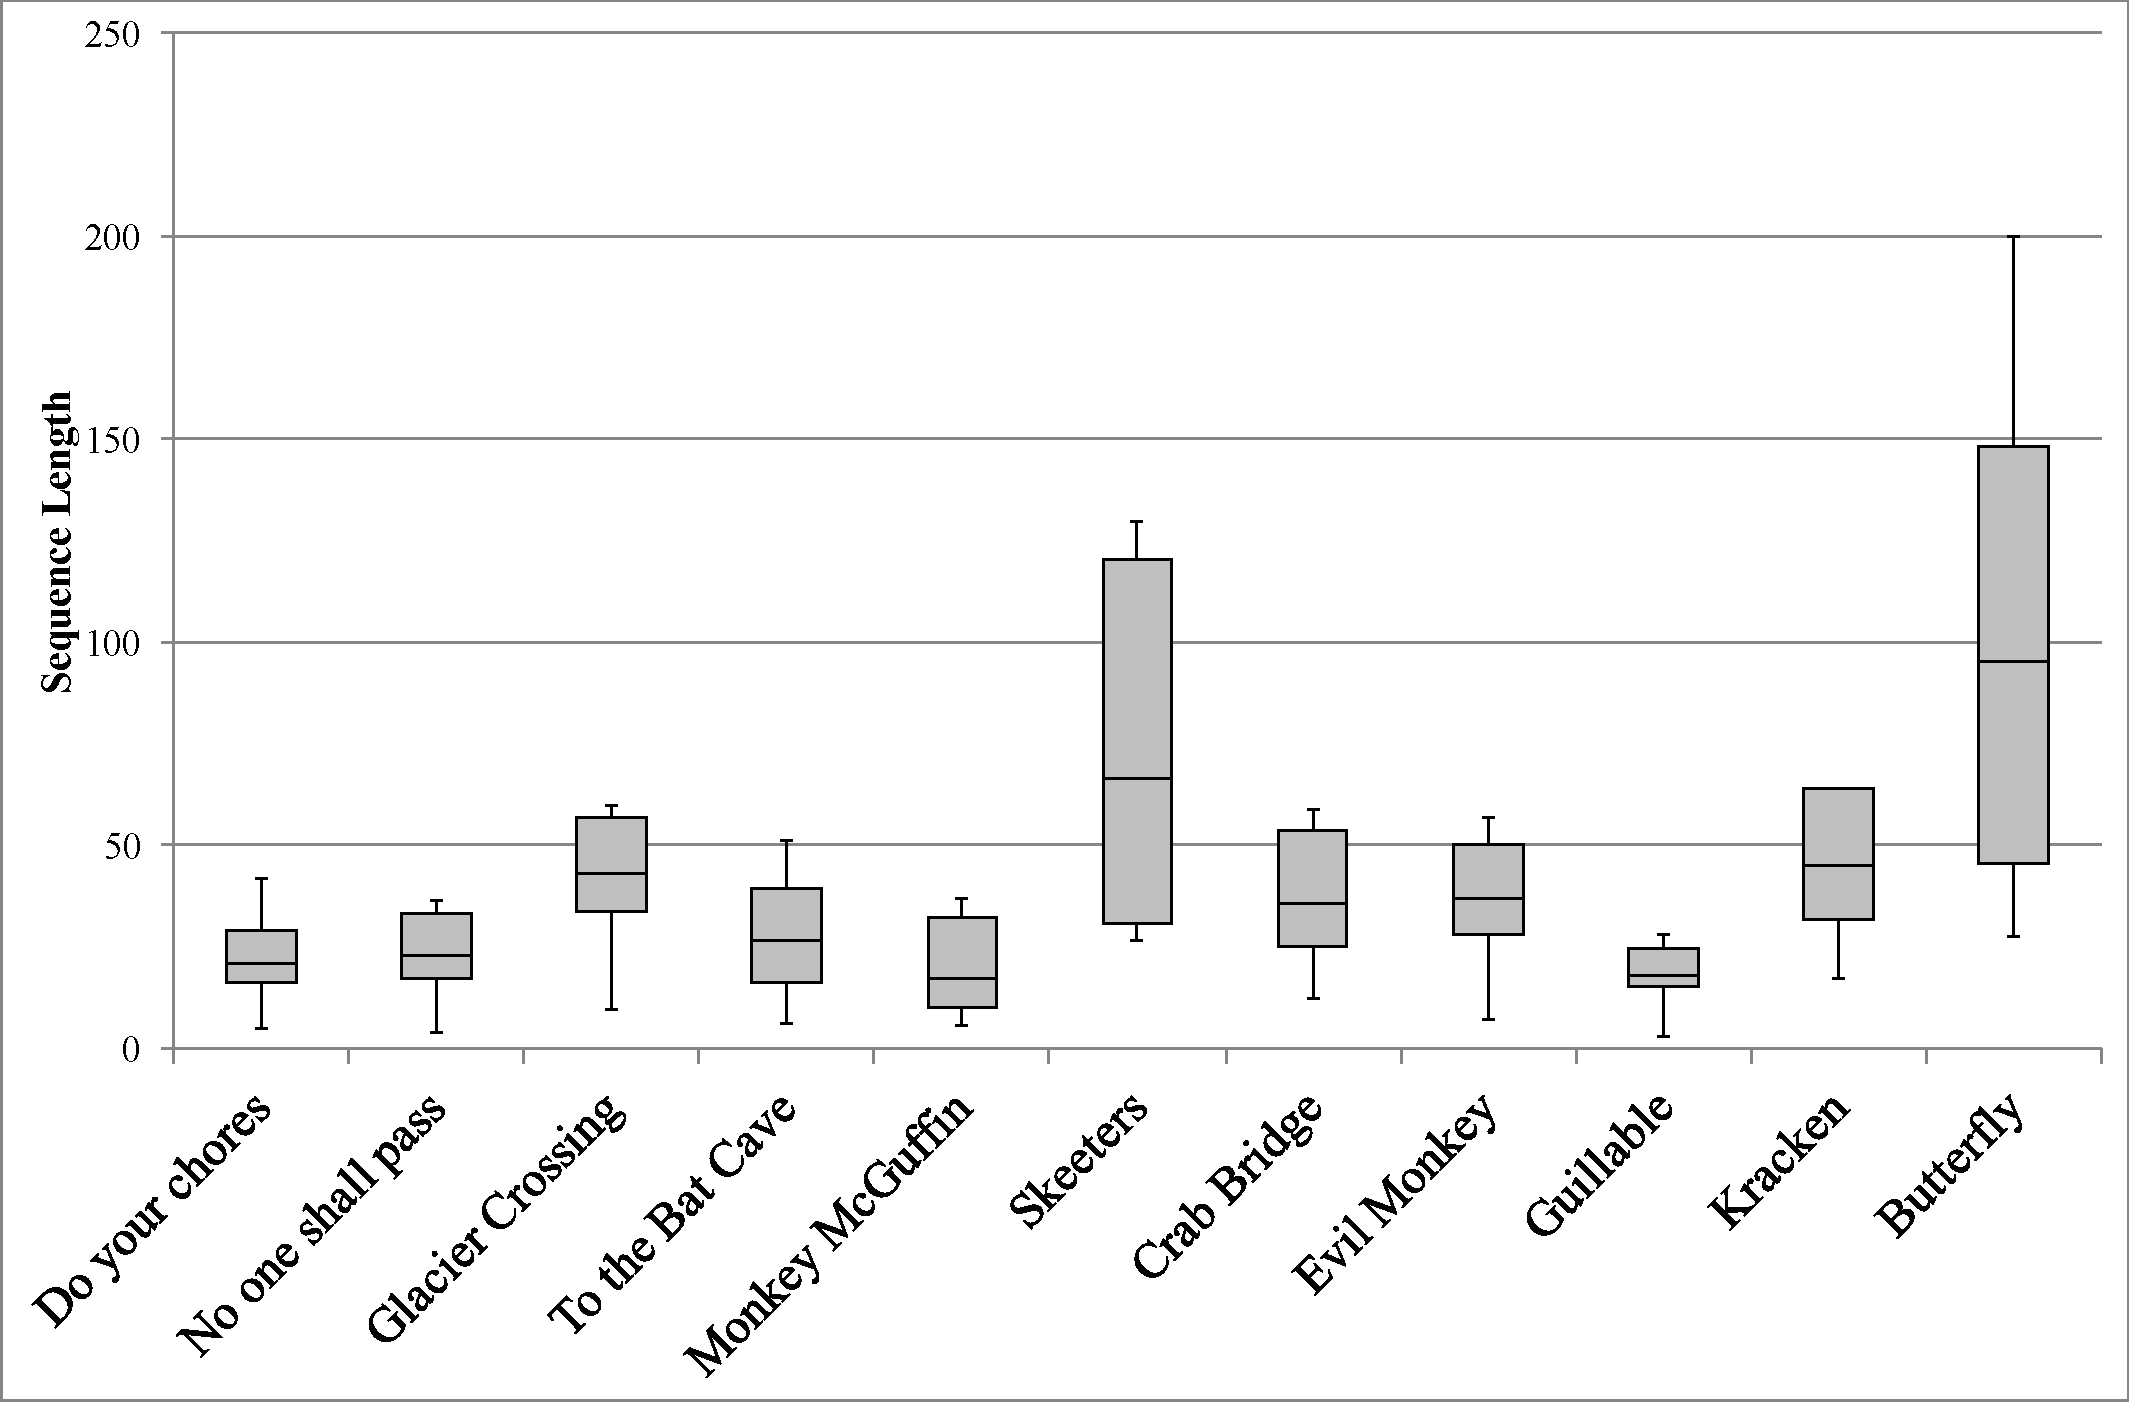
\includegraphics[width=0.9\columnwidth]{figures/boxplot.pdf}
	\caption{Boxplot of Sequence Length in Each Game Level}~\label{fig:boxplot}
\end{figure}

\subsection{Experimental Setup}
First we divide students into two groups, one (\%80) for training and development purposes and the other (\%20) for test and verification.
In the discretization phase, we transformed the log data from slot-and-filler structure each game level into sequences of multinomial variables that can be used as evidence for learning for each student.
In the sequence modeling phase, we use the multinomial sequences of students in the development set (\%80) to train two HMMs that that represent high- and low-performing students.
In the regression phase, we uses the likelihood of students' sequences in order to build a regression model that is predictive of the post-test results.
Finally, we test the regression model on the held-out set (\%20) and report the results.


\subsection{Results}
In order to evaluate our regression model we decided to compare its performance agains two baselines: 1) A regression model that uses success and failure of students in each game level as feature and 2) A regression model that uses the normalized sequence lengths in each game level. 
Our model was able to outperform both baselines regarding to mean absolute error (MAE) and root mean squared error (RMSE). 
Moreover, the correlation and Spearman $\rho$ of our predicted values with the true values were much higher than both baselines. 
Table \ref{tab:results} shows the results.

\begin{table}[tbh]
	\centering
	\begin{tabular}{@{}lllll@{}}
		\toprule
		\begin{tabular}[c]{@{}l@{}}\textbf{Predictive Features}\end{tabular}            & \begin{tabular}[c]{@{}l@{}}\textbf{$R$}\end{tabular} & \begin{tabular}[c]{@{}l@{}}\textbf{$\rho$}\end{tabular} & \begin{tabular}[c]{@{}l@{}}\textbf{MAE}\end{tabular} & \textbf{RMSE}\\ \midrule
		\begin{tabular}[c]{@{}l@{}}Sequence Length (Normal)\end{tabular} & 0.15                                                     & 0.35                                                 & 2.93                                                          & 3.61 \\
		Success / Failure                                                      & 0.02                                                     & 0.16                                                 & 3.21                                                          & 4.08 \\
				\algname ($K=2, H=1$)                                                                                                        & 0.17                                                 &   0.25                                                        &
				3.60 & 3.10 \\ 
		\textbf{\algname ($K=2$)}                                                      & \textbf{0.55}                                                     & \textbf{0.51}                                                 & \textbf{2.84}                                                          & \textbf{3.35} \\ \bottomrule
	\end{tabular}
	\caption{The results of predicting post-test scores using three different feature sets.}~\label{tab:results}	
\end{table}

In Table \ref{tab:results} we reported two versions of the \algname algorithm. 
The HMM with only one state ($H=1$) represents the model with no memory that only considers the distribution of different observations in a sequence (similar to Gaussian Mixture Models) in order to demonstrate the effect of our discretization step.
The best performing model however, learns the best number of states for each game level based on the training examples and outperforms the model with only one state.
The $K=2$ here refers to the number of HMMs we learn for each game level: one for high-performing students and one for low-performing students. 

In order to evaluate the significance of our results, we calculated the absolute difference between the true and predicted value for each student in our heldout set.
We used paired onesided t-test (n=15) for judging the significane of the improvement over MAE and RMSE.
Unfortunately, the improvement was not significant ($p=0.20$ the Success/Failure baseline and $p=0.26$ the Sequence Length baseline). Figure~\ref{fig:regression} shows the true values vs. predicted values using LASSO regression along with the regression line and \%95 confidence interval.

The regression model also provides us with an insight into how important each game level is in distinguishing between high- and low-performing students. Table \ref{tab:regrweights} shows the weights of each game level in the best perfoming model.
As it is shown in the table, game level 11 (\textit{You Kraken Me Up!} -- screenshot Figure~\ref{fig:figurekracken}), has the highest weight in the regression model. 
This can be interpreted as the difference between the sequence of student interactions in this game level has the highest factor in distinguishing between high- and low-performing students.

\begin{table}[b]
	\centering
	\begin{tabular}{ll}
		\hline
		\textbf{Game Level} & \textbf{Weight} \\ \hline
		You Kraken Me Up!   & 1.686                               \\
		Skeeterz            & 1.059                               \\
		Evil Monkeys        & 1.053                               \\
		To the Bat Cave     & 0.855                               \\
		None Shall Pass     & 0.417                               \\
		...                 &                                    
	\end{tabular}
	\caption{Weights of each game level in the best performing model.}
	\label{tab:regrweights}	
\end{table}


\begin{figure}
	\centering
	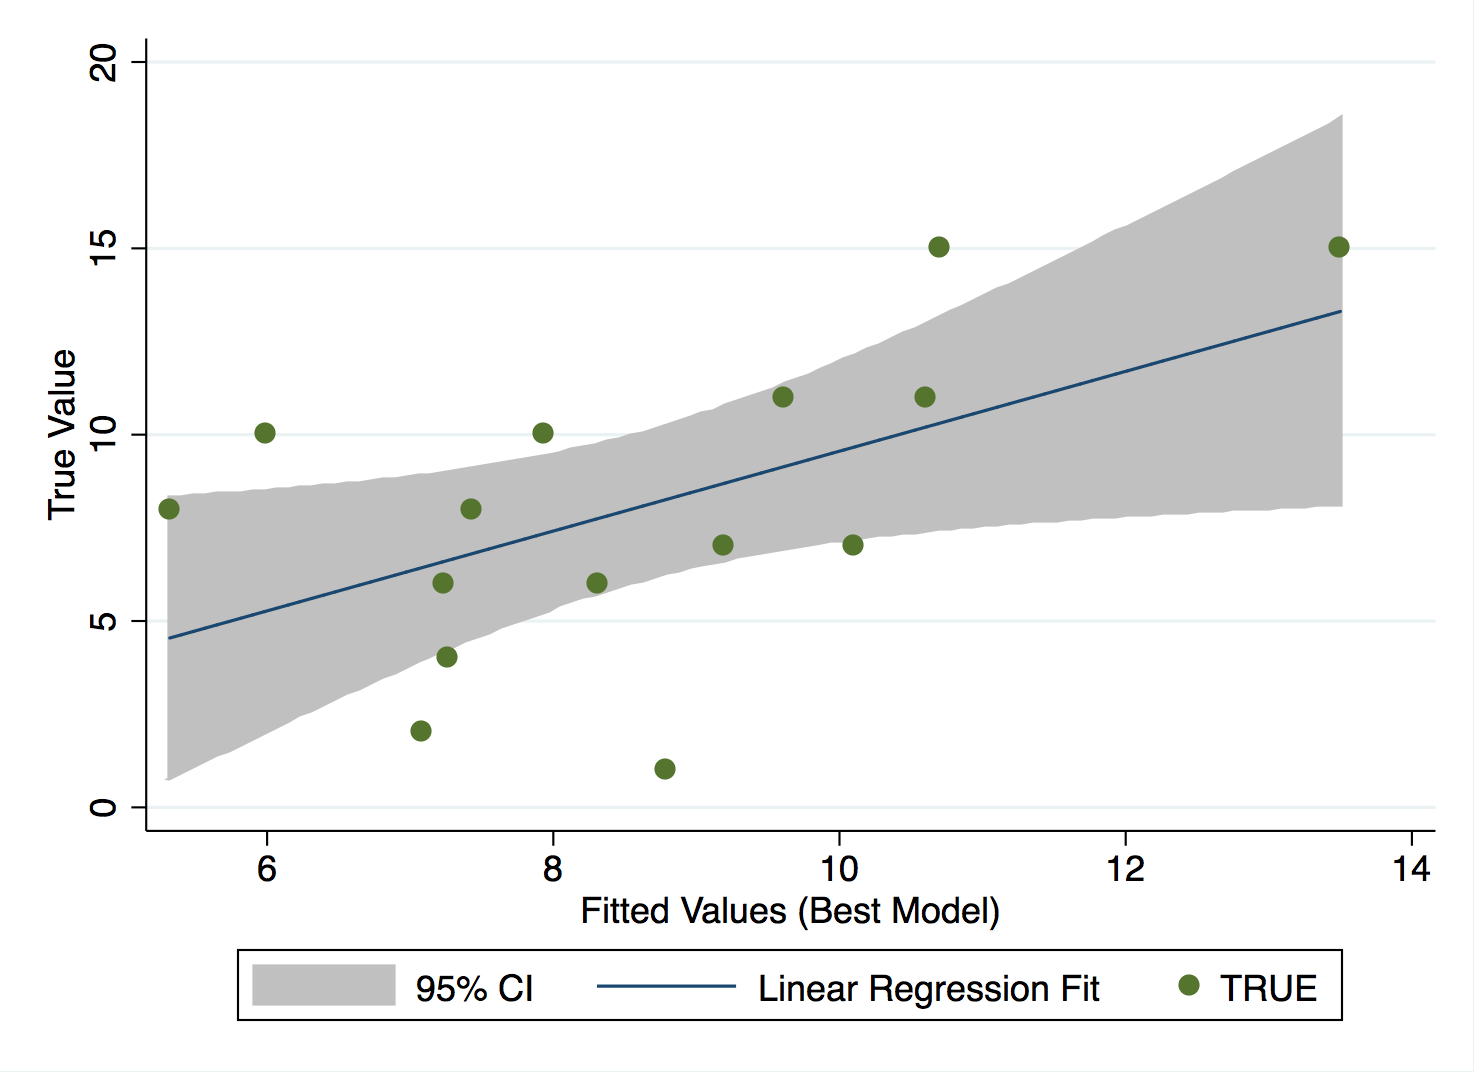
\includegraphics[width=0.9\columnwidth]{figures/regression.png}
	\caption{Results of predicting the post-test scores of the held-out set along with the regression line and \%95 interval.}~\label{fig:regression}
\end{figure}

	
\begin{figure*}
	\centering
	\begin{subfigure}[b]{.48\textwidth}
		\centering
		\resizebox{1\textwidth}{!}{
			
			\begin{tikzpicture}[->,>=stealth',shorten >=0pt,auto,node distance=.3cm,main node/.style={draw, ellipse}]
			\node[main node] (1) {S0};
			
			\node[main node] (3) [right=of 1, xshift=2cm, yshift=1cm]{S1};
			\node[main node] (2) [below=of 3, yshift=-1.3cm, xshift=.5cm, fill=lightgray]{\texttt{UsedEsploda}};
			
			\node[main node] (5) [right=of 3, xshift=3.5cm, yshift=-.5cm, fill=lightgray]{\texttt{MoveCombo\_0}};
			\node[main node] (4) [above=of 5, yshift=1.5cm]{S2};
			\node[main node] (6) [below=of 5, fill=lightgray]{\texttt{UsedGluumi}};
			\node[main node] (7) [below=of 6, fill=lightgray]{\texttt{MoveObject\_0}};
			
			\node[main node] (10) [right=of 4, fill=lightgray, xshift=3cm]{\texttt{MoveCombo\_4}};
			\node[main node] (9) [above=of 10, fill=lightgray]{\texttt{MoveCombo\_2}};
			\node[main node] (8) [above=of 9, fill=lightgray]{\texttt{MoveCombo\_1}};
			\node[main node] (11) [below=of 10, fill=lightgray]{\texttt{MoveCombo\_5}};
			\node[main node] (12) [below=of 11, fill=lightgray]{\texttt{Failure}};
			\node[main node] (13) [below=of 12, fill=lightgray]{\texttt{Success}};
			
			\path[thick]
			(1) edge [loop above] node [auto] {0.70} (1)
			
			(1) edge [out=-70,in=180] node [auto] {0.95} (2)
			(1) edge [out=40,in=180] node [auto] {0.28} (3)
			(3) edge [loop above] node [auto] {0.81} (3)
			
			(3) edge [out=-5,in=180] node [auto] {0.34} (5)
			(3) edge [out=-20,in=180] node [auto] {0.30} (6)
			(3) edge [out=-45,in=180] node [auto] {0.29} (7)
			(4) edge [loop above] node [auto] {0.66} (4)
			(3) edge [out=45,in=180] node [auto] {0.11} (4)
			(4) edge [out=220,in=10] node [auto] {0.29} (3)
			
			(4) edge [out=45,in=180] node [auto] {0.12} (8)
			(4) edge [out=20,in=180] node [auto] {0.12} (9)
			(4) edge [out=10,in=180] node [auto] {0.08} (10)
			(4) edge [out=0,in=180] node [auto] {0.10} (11)
			(4) edge [out=-20,in=180] node [auto] {0.19} (12)
			(4) edge [out=-45,in=180] node [auto] {0.32} (13);
			
			
			\end{tikzpicture}
		}
		
		\caption{High Performing}~\label{fig:highhmm}
	\end{subfigure}\quad
	\begin{subfigure}[b]{.48\textwidth}
		\centering
		\resizebox{1\textwidth}{!}{
			\begin{tikzpicture}[->,>=stealth',shorten >=0pt,auto,node distance=.3cm,main node/.style={draw, ellipse}]
			\node[main node] (1) {S0};
			
			\node[main node] (3) [right=of 1, xshift=2cm, yshift=1cm]{S1};
			\node[main node] (2) [below=of 3, yshift=-1.3cm, xshift=.5cm, fill=lightgray]{\texttt{UsedEsploda}};
			\node[main node] (13) [below=of 2, fill=lightgray]{\texttt{MoveObject\_0}};
			
			\node[main node] (5) [right=of 3, xshift=3.5cm, yshift=-.5cm, fill=lightgray]{\texttt{MoveCombo\_0}};
			\node[main node] (4) [above=of 5, yshift=1.5cm]{S2};
			\node[main node] (6) [below=of 5, fill=lightgray]{\texttt{MoveCombo\_5}};
			\node[main node] (7) [below=of 6, fill=lightgray]{\texttt{UsedGluumo}};
			
			\node[main node] (10) [right=of 4, fill=lightgray, xshift=3cm]{\texttt{MoveCombo\_4}};
			\node[main node] (9) [above=of 10, fill=lightgray]{\texttt{MoveCombo\_3}};
			\node[main node] (8) [above=of 9, fill=lightgray]{\texttt{MoveCombo\_2}};
			\node[main node] (11) [below=of 10, fill=lightgray]{\texttt{Failure}};
			\node[main node] (12) [below=of 11, fill=lightgray]{\texttt{Success}};
			
			\path[thick]
			(1) edge [loop above] node [auto] {0.76} (1)
			
			(1) edge [out=-60,in=180] node [auto] {0.43} (2)
			(1) edge [out=40,in=180] node [auto] {0.22} (3)
			(1) edge [out=-85,in=180] node [auto] {0.55} (13)
			(3) edge [out=220,in=10] node [auto] {0.12} (1)
			
			(3) edge [loop above] node [auto] {0.78} (3)
			
			(3) edge [out=-5,in=180] node [auto] {0.55} (5)
			(3) edge [out=-20,in=180] node [auto] {0.06} (6)
			(3) edge [out=-45,in=180] node [auto] {0.31} (7)
			(4) edge [loop above] node [auto] {0.71} (4)
			(3) edge [out=45,in=180] node [auto] {0.08} (4)
			(4) edge [out=220,in=10] node [auto] {0.20} (3)
			
			(4) edge [out=45,in=180] node [auto] {0.19} (8)
			(4) edge [out=20,in=180] node [auto] {0.10} (9)
			(4) edge [out=10,in=180] node [auto] {0.14} (10)
			(4) edge [out=0,in=180] node [auto] {0.19} (11)
			(4) edge [out=-20,in=180] node [auto] {0.33} (12);
			
			\end{tikzpicture}
		}\\
		\caption{Low Performing}~\label{fig:lowhmm}
	\end{subfigure}
	\caption{Learned Transition Models for One of the Game Levels}~\label{fig:highvslow}
\end{figure*}

\subsection{Discussion and Limitations}
In this study we aimed to explore the effectiveness of data-driven methods for student modeling in educational games. 
To demonstrate the effectiveness of our framework, we used features from it to predict the post-test results using a regression model and showed improvement over two  baselines based on intuition.

As it is reported in the results section, the improvement results were not significant. We investigated this problem in more depth and we believe that the reason we could not achieve significant improvement was mainly because we tested the algorithm on a small dataset.
Our heldout set contains only 15 students and a few of them achieved poor performance results in the post-test while successfully finishing most of the game levels.
This effect is clearly observable in Table \ref{tab:results} where a 0.4 improvement in correlation over the first baseline resulted in 0.09 and 0.26 improvement over MAE and RMSE respectively. 
This observation could raise a question for the utility of similar data-driven models.
However, we believe that using a larger data set will lower the negative effect of such students in the future.

Another limitation of our approach is that our student performance clustering phase uses the post-test scores (independent variable) to divide students into high- and low-performance groups. 
In order to avoid using information from the independant variable to calculate the features of our regression model, we are using a \%80-\%20 split to validate the results instead of for example using a 10-fold cross validation. 

The difference in predictive performance between game levels is likely related to game design. 
Some game levels are designed to introduce game tools and techniques while others are created to present choices to players aligned with math proficiency.
We believe the source of difference is mainly due to the fact that finding the solution to later game levels requires mastery in all three major subskills targetted by the game design.

On the other hand, predicting post-test scores was not the only reason for designing the pipeline.
We were also seeking for a descriptive model that can give us insight into low-level patterns in student movements. 
This was the main idea behind using HDP-HMMs in the sequence modeling phase and our hypothesis that high-performing and low-performing sudents have different sequential patterns. 

Figure~\ref{fig:highvslow} shows the difference between two HMMs learned for one of the game levels.
In this game level in the initial state, students are presented with composite objects and they have to use the \texttt{Esploda} tool to convert them into single unit objects. 
Then, they have to use the \texttt{Gluumi} tools to convert the single unit objects into composite objects that fit the designated area. 
And finally, they have to move the composite object they have created into the designated area.
For comparison purposes, we are showing a three state HMM for both high- and low-performing students and removed the edges that had the probability below 0.05. 
Figure~\ref{fig:highhmm} represents the HMM for high-performing students. 
The three latent states, $S_{0-2}$ can be interpreted as sequential steps, that students took for solving this problem. As illustrated in Figure~\ref{fig:highhmm}, high-performing students follow the expected path of using the \texttt{Esploda} tool in $S_0$, using the \texttt{Gluumi} tool in $S_1$, and then moving the composite objects into the designated areas \texttt{MoveCombo\_{ClusterID}} untill they successfully finish the game.
On the other hand, low-performing students (Figure~\ref{fig:lowhmm}) do not necessarily follow the expected path and the probability of moving object into the outlier clusters (\texttt{MoveObject\_0 and MoveCombo\_0}) is also higher in each state for low-performing students.

\section{Conclusion and Future Work}
Modeling student behavior in open-ended environments such as educational games is an interesting and complex problem. Particulary data-driven models, can be valuable tools for game designers, educators, and researchers for analyzing how students learn different skills by using their systems.
In this paper, we presented a data analysis framework that is able to learn a model from game activity logs that is predictive of student proficiency with minimum reliance on expert knowledge about the game environment. 
One of the key drawbacks of model-free methods is that their results are difficult to interpret. 
However, the discretization process along with the use of HDP-HMM, makes our model human readable and can give us insight into how student interact with each game level.
Moreover, the parameters of the regression model provides a good intuition about the importance of each game level and its influence in distinguishing between high- and low-performing students.

There are many possible directions for future work. On a lower level we can integrate the discretization and sequence modeling step by designing a new type of Hidden Markov Model that accepts slot and filler sequences as input (work in progress). On a higher level, instead of dividing students into two groups (high- and low-performing), we can use the HMM in order to cluster students \cite{bicego2003similarity,smyth1997clustering} into more groups that might be  more representative of different approaches students follow in order to solve each game level. We can also replace our regression model with a more powerfull ensemble method that considers different subskills in order to integrate features of each game levels in order to predict the post-test scores.

We only used data from \textit{Alice in AreaLand} in order to evaluate our model. However, the model is designed in a way that can model sequence of student actions in other similar gaming environments that use slot-and-filler structures in order to log student interactions with the system. Finally, using our framework we will be able to build a model that detects incorrect strategies or common misconception that can be used in a dynamic hinting system in order to increase player engagement and learning.

\bibliographystyle{SIGCHI-Reference-Format}
\bibliography{references}

\end{document}
